\begin{frame}[fragile]{Proof of Concept: $DP_{WCC}$}
  \begin{itemize}
    \item Develop the algorithm presented before using \textbf{Haskell}
  \end{itemize}
\end{frame}

\begin{frame}[fragile]{Proof of Concept: $DP_{WCC}$}
  \begin{itemize}
    \setlength\itemsep{2em}
    \item {\color{light}Develop the algorithm presented before using \textbf{Haskell}}
    \item Conduct empirical analysis to prove suitability of implementation
  \end{itemize}
\end{frame}

\begin{frame}[fragile]{Proof of Concept: $DP_{WCC}$}
  \begin{itemize}
    \setlength\itemsep{2em}
    \item {\color{light}Develop the algorithm presented before using \textbf{Haskell}}
    \item {\color{light}Conduct empirical analysis to prove suitability of implementation}
    \item Write an \textbf{article} and present the results in \textbf{PROLE21 Conference}~\cite{prole:2021:017}
  \end{itemize}
  \begin{textblock*}{7cm}(7cm,6cm) % {block width} (coords)
    \fbox{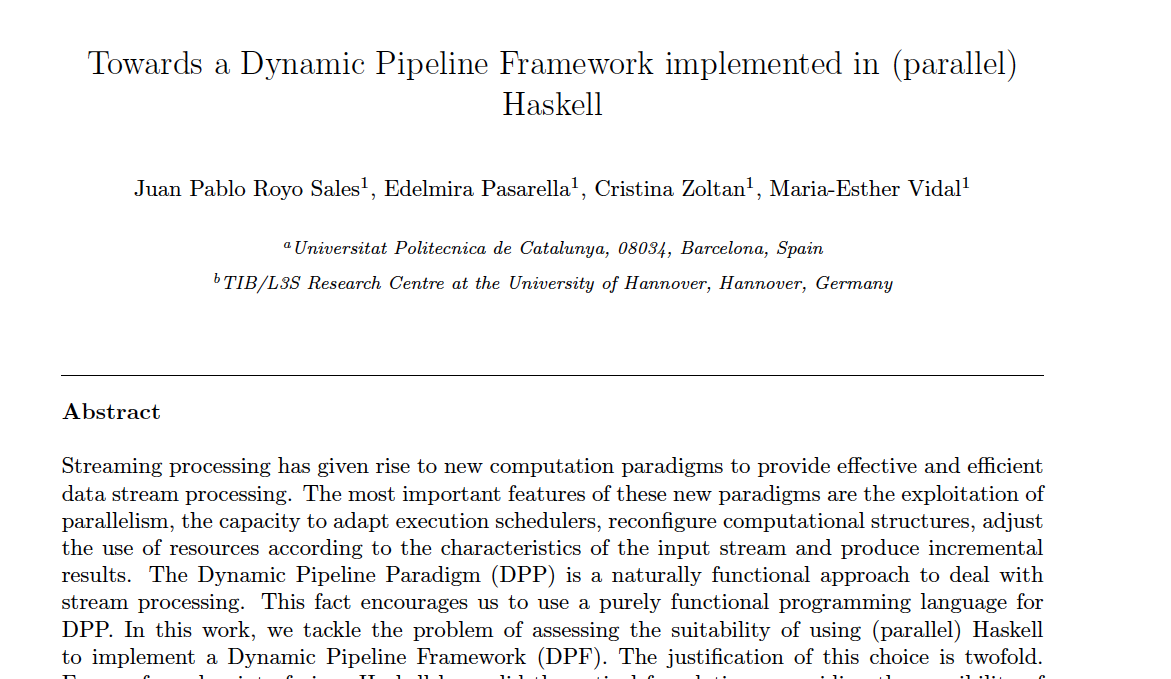
\includegraphics[width = 0.7\textwidth, height = 0.3\textheight]{paper-prole}}
  \end{textblock*}
\end{frame}

% \begin{frame}[fragile]{Proof of Concept: $DP_{WCC}$ - Empirical Evaluation}
%   \begin{block}{Research Questions}
%     \begin{itemize}
%           \item Does $\dpwcc$ in Haskell support the dynamic parallelization level that $\dpwcc$ requires?
%           \item Is $\dpwcc$ in Haskell competitive compared with default implementations on base libraries for the same problem?
%           \item Does $\dpwcc$ in Haskell handle memory efficiently?
%       \end{itemize}        
%   \end{block}
%   \begin{block}{Experiments}
%     \begin{itemize}
%       \item \textbf{Implementation Analysis}: Measure and analyze Total execution time, MUT time and GC Time.
%       \item \textbf{Benchmark Analysis}: Compare $DP_{WCC}$ with \mintinline{haskell}{Data.Graph} $WCC$ execution times:
%       \begin{itemize}
%         \item Using \mintinline{haskell}{ criterion } library.
%         \item Diefficency metric $\mathtt{dief@t}$ (\textit{diepfy} tool) to measure incremental results.
%       \end{itemize}
%       \item \textbf{Performance Analysis}: Thread and Memory allocation analysis.
%     \end{itemize}
%   \end{block}
% \end{frame}

\begin{frame}[fragile]{Proof of Concept: $DP_{WCC}$}
  \begin{block}{Conclusions}      

  \begin{itemize}
    \setlength\itemsep{2em}
    \item \textbf{Robustness and Suitability} of the DP-Haskell 
    \item \textbf{Ability to generate Incremental results} has been shown by $\mathtt{dief@t}$ metrics
    \item \textbf{Satisfactory Performance results} with an adequate Memory allocation and Execution times. 
  \end{itemize}
\end{block}
\end{frame}

